\subsection{Graphical User Interface}

The Java Server's User Interface is constituted by two parts: the Main Window and the Configuration Dialog.

\subsubsection{Main Window}

The Main Window has two sections: the first allows the connection set-up with the panstamp server while the second displays the overall state of each module in the network (see Figure ~\ref{java-server-main}). 
% latex does not insert anything
To establish a connection, the user has to select the serial port, which the panstamp is attached to, and the corresponding baud-rate. Once the connection is set up, the "connect" button is substituted by a "disconnect" button. The user can disconnect and connect the panstamp at any time. 
% For example if one decides to change the used serial port. 
If the Java server does not detect a device (module) in any of the serial ports, the "connect" button will be unavailable (i.e. grayed out). To prevent the user from constantly restarting the server, we implemented a refresh button, which can be pressed at any time. When a device is finally detected, both options (connect and disconnect) will be available for that device.

In the second section of the Main Window, the overall state of each device (module) in the network is shown in a table (see Figure ~\ref{java-server-main}). 
Among the data displayed are: the name of the module's personality, the direct neighbour, the actual state, the last corresponding time to the server and the battery state. 

For this project, we implemented three standard personalities named "Paul" (default personality), "Tanja" and "Mama".

After the start-up and before users interact with the modules, these devices won't have a direct neighbour so the field 'Neighbour' initial value is 'none'. When a module detects a neighbor module, the field 'Neighbour' will display the name of the detected neighbor's personality.
 
The field 'State' indicates how persistently a module is being kicked.
Before users interact with the modules, each device is in "stand-by". After the first interaction, the state will change to "first contact"; then, the following states are "played" and "played (hard)". Each device (module) goes through all possible stages before reaching "played (hard) state; thus, a direct change from "first contact" to "played (hard)" is not possible.

The forth field 'last seen' indicates the time when the last communication between device and server has been.

The last row in the table, 'Battery', indicates the charge of the Li-Po battery and the two possible states are: "OK" and "low battery".

To reflect new detected modules in the network and changes in the devices' status, the information on the table is periodically updated; the table's refresh rate is configurable. 
The update process is implemented using a timed thread, which is periodically checking the modules' data and altering the shown information accordingly. In case the battery state was set to "low battery" or the last received message was received long ago (when 'last seen' value surpasses a configured threshold), the main window will change the background of the device's  personality entry in the table to red to alert the user. 
\begin{figure}[h!]
 \centering
 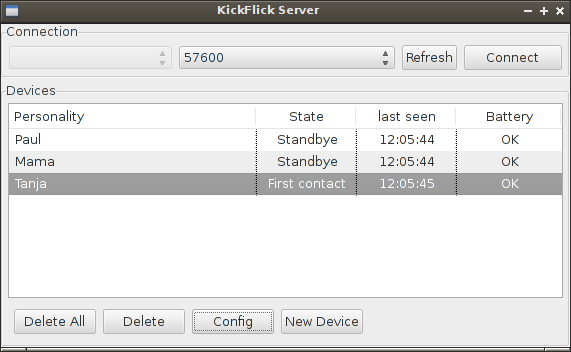
\includegraphics[width= 0.5\textwidth, clip=true  ,keepaspectratio=true]{./pic/java-server-main.png}
 % java-server-main.png: 0x0 pixel, 0dpi, nanxnan cm, bb=
 \caption{Main Window}
 \label{java-server-main}
\end{figure}

If the server detects a new module in the network, the user can select it in the device-table and open a configuration dialogue by either pressing the configuration button (located on the bottom of the table) or by clicking on the intended table's item. The configuration dialogue will then be opened to allow the configuration of this particular device's personality.

\subsubsection{Configuration Dialogue}

The Configuration Dialogue provides all the information about the selected module's state and allows the configuration of the device's personality. 

The user can customize a personality or select one among the predefined personalities. But if the user creates a personality and then selects a predefined one, all the changes made so far will be overridden by the predefined personality. 

To cancel all changes, the user has to click the ''close'' button located on the bottom-right corner of the Dialogue Window (see Figure ~\ref{fig:java-server-config01}).   

In the Configuration Dialogue, the personality's settings are distributed in three different tabs. The tab ''Basic'' (see Figure ~\ref{fig:java-server-config01}) contains the personality's name, the addresses of the two nodes that constitute the entity and a table with all the possible action keys. Only the checked keys will be enabled in the entity; that is, the entity will only react to a certain action key if the latter has a check next to it in the table. Every key can be enabled and disabled by the user. 

By clicking on a device in the table of the main window, this first view of the configuration window opens. In the Default Configuration part of the window the chosen device will be shown with its device name. Because the user can overwrite the name of a personality, it was necessary to show the actuators and the sensors ID.
Furthermore the actual state of the device is prompted so that the user can change the behaviour of a device in a special state. 


\begin{figure}[h!]
 \centering
 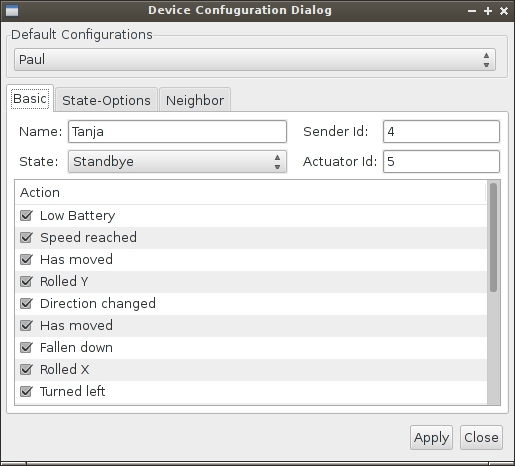
\includegraphics[width= 0.5\textwidth, clip=true  ,keepaspectratio=true]{./pic/java-server-config01.png}
 % java-server-main.png: 0x0 pixel, 0dpi, nanxnan cm, bb=
 \caption{Configuration Dialog, 1st Tab}
 \label{fig:java-server-config01}
\end{figure}

In the second tab of the Configuration Window the "Reaction Options" are set.
So the window is separated in an upper and a lower part. In the upper one the behaviour of the device can be set in the Standby (default) state. A personality's behaviour is interpolated by four objects: Once, there is a pattern (like blinking, fading, rainbow, ... ). This pattern needs two colours to switch between. At least, the behaviour needs a time (duration) for how long a pattern is.
In the lower part all other states can be manipulated.   


\begin{figure}[h!]
 \centering
 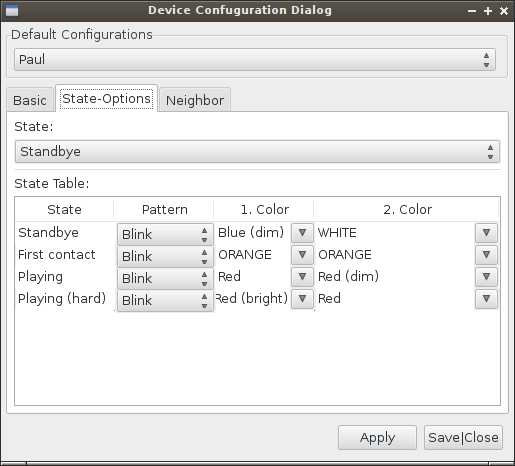
\includegraphics[width= 0.5\textwidth, clip=true  ,keepaspectratio=true]{./pic/java-server-config02.png}
 % java-server-main.png: 0x0 pixel, 0dpi, nanxnan cm, bb=
 \caption{Configuration Dialogue, 2nd Tab}
 \label{fig:java-server-config02}
\end{figure}


Finally, the third tab labelled ''Neighbor'' displays the actions to be performed when the entity detects a neighbor (see Figure ~\ref{fig:java-server-config03}). The table shows the personality of each entity that has been detected by the server. However, if an entity has a preset personality, it will not be displayed in this tab since its reaction towards a neighbour is already defined and is not configurable. 

In this tab, the user can set the pattern and colors that the entity and its found neighbor will display. For instance, according to the settings in Figure ~\ref{fig:java-server-config03}, if the entity ''Mama'' finds ''Tanja'', both entities will exhibit a blink pattern with white and black. On the other hand, when ''Tanja'' finds ''Mama'', the two entities will again display a blink pattern but with different colors, namely red and blue. 

In order to save the changes made to the personality's settings, the user has to press the ''save|close'' button. Otherwise, if just the ''save|close'' button were pressed, no changes would be written and the device would keep the settings it had before the configuration process.

\begin{figure}[h!]
 \centering
 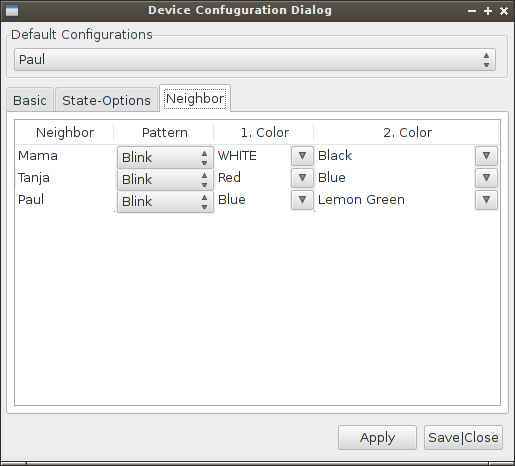
\includegraphics[width= 0.5\textwidth, clip=true  ,keepaspectratio=true]{./pic/java-server-config03.png}
 % java-server-main.png: 0x0 pixel, 0dpi, nanxnan cm, bb=
 \caption{Configuration Dialog, 3rd Tab}
 \label{fig:java-server-config03}
\end{figure}

\subsubsection{Interface Architecture}
The interface was created with the swt widget toolkit from eclipse. %insert cite
To periodically update the device table, the main window uses a swt timerevent. Every event-based action, like button clicks or selection were also implemented with the built-in event-listener structure of the swt toolkit. %insert cite again

When the dialogue is opened, the entity will be passed as a parameter in the constructor, the dialogue will then create the interface and afterwards read the entity's settings %Daniel, what do you mean by dialogue here? The Configuration Dialogue?

Every change will be written to a new device class instance, witch chares the same configuration as the selected device, so that the if the users closes the configuration dialog via clicking the "save|close" button this instance replaces the previously selected device.

The interface was designed to be highly felxible, if one decides to add new colors or add an extra state to the device and personality structure, the inferface widgets don't need to be changed. They are dynamicly created at startup and therefor hold all availably informations.
% vim: spell spelllang=en_gb 
